%% LyX 2.1.1 created this file.  For more info, see http://www.lyx.org/.
%% Do not edit unless you really know what you are doing.
\documentclass[10pt,english,paper=a4,fontsize=10pt]{scrartcl}
\usepackage[latin9]{inputenc}
\usepackage{color}
\usepackage{babel}
\usepackage{amsthm}
\usepackage{amsmath}
\usepackage{amssymb}
\usepackage{esint}
\usepackage[authoryear]{natbib}
\usepackage[unicode=true,
 bookmarks=true,bookmarksnumbered=true,bookmarksopen=false,
 breaklinks=false,pdfborder={0 0 0},backref=false,colorlinks=true]
 {hyperref}
\hypersetup{
 urlcolor=webbrown,linkcolor=Blue,citecolor=webgreen}

\makeatletter
%%%%%%%%%%%%%%%%%%%%%%%%%%%%%% Textclass specific LaTeX commands.
\RequirePackage{todonotes}
  \theoremstyle{definition}
  \newtheorem{defn}{\protect\definitionname}
\theoremstyle{plain}
\newtheorem{thm}{\protect\theoremname}
  \theoremstyle{plain}
  \newtheorem{prop}{\protect\propositionname}
 \theoremstyle{definition}
  \newtheorem{example}{\protect\examplename}

%%%%%%%%%%%%%%%%%%%%%%%%%%%%%% User specified LaTeX commands.
% article example for classicthesis.sty
 % KOMA-Script article 
\usepackage[nochapters]{classicthesis}% nochapters
\let\oldtitle\title\renewcommand{\title}[1]{\oldtitle{\rmfamily\normalfont\spacedallcaps{#1}}}
\let\oldauthor\author\renewcommand{\author}[1]{\oldauthor{\spacedlowsmallcaps{#1}}}
\date{}

\definecolor{Blue}{cmyk}{1, 0.878, 0, 0}
\usepackage{tikz}
\usepackage{pgfplots}
\usepackage{amssymb}

\let\marginpar\oldmarginpar%fix for todo notes

\@ifundefined{showcaptionsetup}{}{%
 \PassOptionsToPackage{caption=false}{subfig}}
\usepackage{subfig}
\makeatother

  \providecommand{\definitionname}{Definition}
  \providecommand{\examplename}{Example}
  \providecommand{\propositionname}{Proposition}
\providecommand{\theoremname}{Theorem}

\begin{document}

\title{Physician Information Acquisition In a Dynamic Setting}


\author{Rud Faden}

\maketitle
\tableofcontents{}



\global\long\def\argmax{\operatornamewithlimits{arg\, max}}

\begin{abstract}
In this project, I examine provider and patient demand for information
in a dynamic model where the diagnostic precision is assumed to be
related to physician effort, and effort is noncontractible. In each
period where the patient and physician interact, the physician gathers
information about the patient, and the diagnostic precision is increased.
Therefore, optimal physician effort decreases as the physician and
patient tie increases. As the physician is unobserved, the insurer
compensates the physician by the average effort in the physician population
and physician will not provide an optimal level of diagnostic precision
in the in the first encounters with a new patient. Therefore the switching
cost of the patient increases as the tie with the physician lengthens.
This model explains (i) why the cost is negatively related with patient,
physician ties and (ii) also introduces the concept of an \textquotedblleft%
information
trap\textquotedblright, where competition is deceasing in the patient
physician tie as switching cost increases. Increases.
\end{abstract}

\section{The Patients Utility}

Following \citet{Rochaix1989}, the patient has a utility function
\begin{eqnarray*}
U & = & u(t,s):\, T\times S\rightarrow\mathbb{R}
\end{eqnarray*}


where $t$ is treatment, $s$ is disease variable classified by its
severity of illness, where both $t$ and $s$ traverse a real line.
It is assumed that the utility function has both increasing and decreasing
parts to capture the negative effects of both under and over treatment.
It is further assumed that the disutility of moving away from the
optimum is increasing in $s$, such that the patient is more \emph{risk-sensitive}
for higher values of $s$. 
\begin{defn}
\label{def:risk-sensitivity}Assuming that the decision problem has
a unique solution $t^{*}(s)$, and for $s'>s$, $u(t^{*}(s),s)=u(t^{*}(s'),s')$.
Then for $t^{*}(s)>t_{1}$, $t^{*}(s')>t_{2}$, $t_{2}\ge t_{1}$
and $t^{*}(s')-t_{2}=t^{*}(s)-t_{1}=\Delta t$, the \emph{risk-sensitivity}
is monotonically increasing in $s$, if 
\begin{equation}
0\le u(t^{*}(s),s)-u(t_{1},s)\le u(t^{*}(s'),s')-u(t_{2},s')\label{eq:risk-sensitivity}
\end{equation}


for all $s$ and $t$, and I write that $u(t_{1},s)\preceq u(t_{2},s')$. 
\end{defn}
The notion of \emph{risk-sensitivity} is illustrated in figure\ref{fig:The-patients-utility}.
\begin{thm}
\label{thm:single-crossing}If the risk sensitivity is increasing
in $s$, then for $s'>s$ $u(t,s)$ has a single crossing property
in $(s,t)$\end{thm}
\begin{proof}
Let $t'=t^{*}(s')$ and $t=t^{*}(s)$. Given definition\ref{def:risk-sensitivity},
it is clear that $t'\ge t_{2}>t\ge t_{1}$. Therefore I can rewrite
\eqref{eq:risk-sensitivity} as 
\begin{equation}
u(t',s')-u(t_{2},s')\ge u(t,s)-u(t_{1},s)\ge0\label{eq:increasing-differences}
\end{equation}


\eqref{eq:increasing-differences} clearly have increasing differences
in $s$ and thereby satisfies the single crossing property. 
\end{proof}
The intuition behind theorem\ref{thm:single-crossing}, is that the
marginal change $u(t',\cdot)-u(t,\cdot)$ is larger, when $s$ is
larger. When $u(t,s)$ is differentiable and concave as in figure
\ref{fig:The-patients-utility}, one might note $\partial u(t,s)/\partial t\ge0$
for $t\le t^{*}(s)$ and that for $\partial u(t,s)/\partial t\le0$
for $t\ge t^{*}(s)$. Thereby $\partial u(t,s')/\partial t>\partial u(t,s)/\partial t$
for $t\le t^{*}(s)$ and $\partial u(t,s')/\partial t<\partial u(t,s)/\partial t$
for $t\ge t^{*}(s)$. If $u(t,s)$ is convex, then one might note
that $\partial u(t,s')/\partial t$ crosses $\partial u(t,s)/\partial t$
at most once and from below. 

\begin{figure}
\subfloat[Utility]{\resizebox{0.45\textwidth}{!}{%
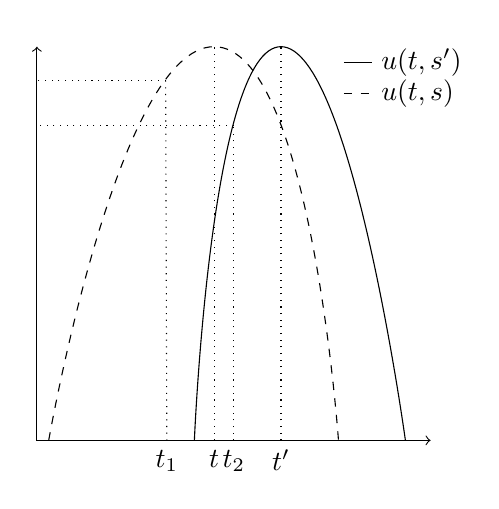
\begin{tikzpicture}[scale=0.5]
\draw[<->] (-3.5,10) node[above]{}--(-3.5,0)--(6.5,0)node[right]{}; 
\draw[dashed] (4.3,8.8)--(5,8.8)node[right]{$u(t,s)$}; 
\draw[] (4.3,9.6)--(5,9.6)node[right]{$u(t,s')$};  
\draw[dashed]  plot[smooth, tension=1.2] coordinates {(-3.2,0) (1,10) (4.16,0)}; \draw  plot[smooth, tension=1.2] coordinates {(0.5,0) (2.7,10) (5.86,0)}; \draw[dotted] (2.7,0)node[below]{$t'$}--(2.7,10); 
\draw[dotted] (1.5,0)node[below]{$t_2$}--(1.5,8); 
\draw[dotted] (1,0)node[below]{$t$}--(1,10); 
\draw[dotted] (-0.2,0)node[below]{$ t_1$}--(-0.23,9.15); 
\draw[dotted] (1.5,8)--(-3.5,8); 
\draw[dotted] (-0.23,9.15)--(-3.5,9.15);
\end{tikzpicture}
}


}\hfill{}\subfloat[Single Crossing]{
%\resizebox{0.45\textwidth}{!}




}

\protect\caption{\label{fig:The-patients-utility}The patients utility functions. If
for the same change in $t$ the loss in utility is smaller for $s$
than for $s'$, when $s<s'$, then I says that risk sensitivity is
increasing in $s$.}
\end{figure}

\begin{prop}
Given that $u(t',s)-u(t,s)$ has a single crossing property in $s$
and that both $S$ and $T$ are well ordered sets, then 
\[
t^{*}(s)=\argmax_{s\in S}u(t,s)
\]


is increasing in $s$. %
\footnote{It should be noted that the assumption of quasisupermodularity is
not needed as the choice space is well ordered (e.i.\ a chain). %
}\end{prop}
\begin{proof}
As both $T$ and $S$ are real lines, then it follows trivially that
they are well ordered. For the rest of the proof see \citet{Milgrom1994}\end{proof}
\begin{example}
A function with the properties defined in theorem\ref{thm:single-crossing}
and definition\ref{eq:risk-sensitivity} and have the form as in
figure\ref{fig:The-patients-utility} is 
\begin{equation}
u(t,s)=c-s{(s-t)}^{2}\label{eq:utility-example}
\end{equation}


where $t,s\in\mathbb{R}^{+}$. Assuming that\eqref{eq:utility-example}
is continuous and twice differential in $t,s$, the derivative $\partial^{2}u(t,s)\big/\partial t\partial s=2s^{2}\ge0$
and~\eqref{eq:utility-example} has increasing differences and thereby
also a single crossing property in $(t,s)$. However,~\eqref{eq:utility-example}
is not supermodular ($\partial^{2}u(t,s)\big/\partial t^{2}=-2<0)$
nor quasisupermodular in $(t,s)$. 
\end{example}

\section{Uncertainty with perfect agency}

In reality however, $s$ is never observed. The level of severity
for the patients is a random variable represented by $S$, characterized
by a subjective cdf. $F(s)$, with density $f(s)$, where $s$ is a
realization of $S$. The expected value of choosing an admissible
treatment intensity$t$ is given by 
\begin{equation}
u(t,S)=E[u(t,s)]=\max_{t}\int_{S}u(t,s)dF(s)\label{eq:expected-utility-prior}
\end{equation}


It is however possible to acquire costly information about $s$ through
medical diagnostics and physician effort. However, for two experiment
$X,Y$ on $S$, it is not a priori certain that one experiment $X$
is necessary more \emph{informative} about $s$ than the experiment
$Y$, where \emph{informative} is to be understood in the way the
posterior decision induced by the experiment $X$ insures greater
expected utility than the decision induced by the experiment $Y$.
Therefore we must introduce an order of information. 


\subsection{Information ordering}
\begin{defn}
\label{def:afflilation} (\citet{Milgrom1982}) For a family of density
functions, let $x\lor s$ denote the component wise maximum and $x\land s$
the component wise minimum. Then $x$ and $s$ are affiliated if,
for all $s$ and $x$
\[
f(s\lor x)f(s\land x)\ge f(s)f(x)
\]

\end{defn}
Affiliation of two random variables are equivalent to the monotone
likelihood ration property, and the intuition behind definition~\ref{def:afflilation}
is that higher signal realization of $x$ makes the probability that
$s$ is large, higher. Similarly small signal realization of $x$
makes the probability of a small $s$ more likely.
\begin{defn}
\label{def:accuracy} (\citet{Acquisition2000}) Given two signals
(experiments) $X^{\eta}$ and $X^{\eta'}$, $X^{\eta'}$ is more accurate
than $X^{\eta}$ if 
\begin{equation}
T(x)=F^{\eta'^{-1}}(F^{\eta}(x\mid s)\mid s)\label{eq:acuracy tranformation}
\end{equation}
 is non decreasing in $s$ for all $x$.

A family of signals $\left\{ X^{\eta}\right\} _{\eta\in E}$ is accuracy
ordered (A-ordered) if a signal with higher index is more accurate
than a signal with lower index. 
\end{defn}
To understand the concept of accuracy, it can be noted that 
\[
T(X^{\eta}\mid s)\sim X^{\eta'}\mid s
\]


Thus a more accurate signal can be obtained from a less accurate signal,
by the transformation $T(X)$. An example is given in example 
\begin{example}
Let  $\eta\in[0,\infty]$and let $S$ be distributed according to
any CDF and let $X_{\eta}\sim\mathbb{U}(s-1/\eta,s+1/\eta)$. Then
for $\eta'>\eta$ 
\[
\frac{\eta'}{2}=\frac{\eta}{2}\left(T^{-1}(x)\right)'\Leftrightarrow T(x)=\frac{\eta}{\eta'}(x-s)+s
\]
 Thus, $T(x)$ transforms $X^{\eta}$ into $X^{\eta'}$ \citep{Persico1996}.
\end{example}
An illustrative example can also be given by applying $\eqref{eq:acuracy tranformation}$
to hypothesis testing. 
\begin{example}
Consider the case where $s$ can take two values $s_{1}<s_{2}$. Let
$X^{\eta}$ be a information structure affiliated with $S$. The optimal
test based on $X^{\eta}$ is given by the rejection region $X^{\eta}>x^{*}$,
such that $s_{1}$ is rejected in favor of $s_{2}$ when $X^{\eta}>x^{*}$.
The probability of a type I error is then $\mathbb{P}(X^{\eta}\le x^{*})=F(x^{*}\mid s_{2})$
and the probability of a type II error is $1-F(x^{*}\mid s_{1})$.
Now given that $X^{\eta'}$ is more accurate than $X^{\eta}$ is is
possible to design a test with the same probability of type I error,
by choosing $x^{**}$ such that $F(x^{**}\mid s_{2})=F(x^{*}\mid s_{2})$
(e.i. \ accept $s_{2}$ if $X^{\eta}\ge x^{**}$). However, since $X^{\eta'}$
is more accurate than $X^{\eta}$, then $x^{**}\ge F^{\eta'^{-1}}(F^{\eta}(x\mid s_{1})\mid s_{1})$.
As $x^{**}$ lies on or, to the right of $x^{*}$ then the test based
on $X^{\eta'}$ is a least as powerful as the test based on $X^{\eta}$
\citep{Lehmann1988,Acquisition2000}.

\begin{figure}
\resizebox{\textwidth}{!}{%
	\begin{tikzpicture}
	%figure 1
		\draw[<->] (0,8) node[above]{}--(0,0)--(8,0)node[right]{};
		
		\draw (2.5,0)node[below]{$s-\frac{1}{\eta}$}--(2.5,2.5)--(6.5,2.5)--(6.5,0)node[below]{$s+\frac{1}{\eta}$};
		\draw (3.5,0)node[below]{$s+\frac{1}{\eta '}$}--(3.5,4)--(5.5,4)--(5.5,0)node[below]{$s+\frac{1}{\eta '}$};
		\filldraw (4.5,0)node[below]{$s$} circle (2pt);
		% Figure 2
		\draw[<->] (11,8) node[above]{}--(11,0)--(19,0)node[right]{};
		\draw (13.5,0)node[below]{$s-\frac{1}{\eta}$}--(13.5,2.5)--(17.5,2.5)--(17.5,0)node[below]{$s+\frac{1}{\eta}$};
		\draw (11,4)node[below,xshift=-15]{$s+\frac{1}{\eta '}$}--(7,4)--(7,6)--(11,6)node[above,xshift=-15]{$s+\frac{1}{\eta '}$};
		%lines 
		\draw[dashed] (13.5,2.5)--(13.5,4)--(11,4);
		\draw[dashed] (17.5,2.5)--(17.5,6)--(11,6);
		\draw (11.5,3)-- (18.5,6.5)node[right]{$T(x)$};
	\end{tikzpicture}
}

\protect\caption{The $T(x)$ transformation}


\end{figure}

\end{example}

\subsection{Demand for information}

Given that we now know, when a test can be considered more informative
than another, I can know turn to the problem of informativeness. 
\begin{thm}
\label{thm:informative} (\citet{Acquisition2000}) Suppose that $X^{\eta}$
and $X^{\eta'}$ are affiliated with $S$ and that $\left\{ X^{\eta}\right\} _{\eta\in E}$
is A-ordered, such that $X^{\eta'}$ is more accurate than $X^{\eta}$.
Then for all utility functions with a single crossing property $X^{\eta'}$
is more informative than $X^{\eta}$.\end{thm}
\begin{proof}
See \citet{Lehmann1988} section 4 and \citet{Karlin1956a} Lemma
3--4 and theorem 1.
\end{proof}
It follows directly from Theorem~\ref{thm:informative} that when
$X^{\eta'}$ is more informative than $X^{\eta}$, then 
\[
\int_{X}\int_{S}u(t,s)dG^{\eta'}(s\mid x)dF(x)\ge\int_{X}\int_{S}u(t,s)dG^{\eta}(s\mid x)dF(x)
\]


\section{The physician problem}

\section{Dynamic setting}

\bibliographystyle{plainnat}
\bibliography{/home/rudfaden/Dropbox/PhD/Bibtexfiles/library}


\end{document}
